% !TEX root = main.tex
\chapter{Analysis}
\label{analysis}



\section{Algorithm Runtime with Constraints active}
Let us look at how long it takes for the SCVX PDG problem to converge under different constraints active.  For K=10 iterations we perform the following

% for
\begin{itemize}
	\item  glideslope constraint
	\item alignment constraint
	\item sigma constraint
	\item omega max constraint
\end{itemize}

\section{Temporal Node Count Variation}
solve planar problem with K = 8 to 50
look at final time dispersions between Ks
look at fuel consumption dispersions...
log final for each iteration... for each K level


\begin{table}[ht]
\caption{Computation Time (s)}
\centering 
\begin{tabular}{c c c c c} 
\hline\hline \\[0.5ex] 
K & Min & Max & Mean & Stdev \\ 
\hline \\
$10$    &$0.875 $   &$1.771 $  &$1.3023  $  &$0.29$  \\ 
$15$    &$1.331 $   &$2.713 $  &$2.2504  $  &$0.365$  \\ 
$20$    &$2.289$    &$2.986$   &$2.618  $   &$0.230$  \\ 
$30$    &$ 3.38 $   &$4.708 $  &$4.1419  $  &$0.363$  \\ 
$40$    &$4.587 $   &$5.499 $  &$4.9056  $  &$0.257$  \\ 
$50$    &$6.814 $   &$8.637 $  &$7.7515  $  &$0.688$  \\[1ex] 
\hline
\end{tabular}
\label{table:tableplanar}
\end{table}







\begin{figure}[!htbp] 
\label{}
  \centering
  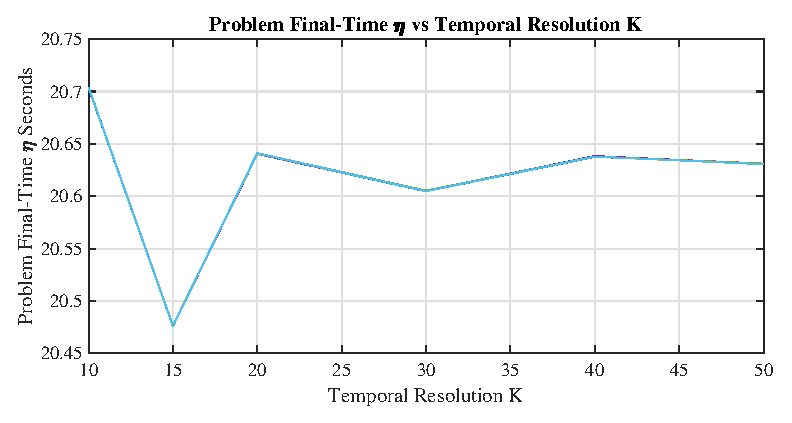
\includegraphics[width=\textwidth]{figs/etavsK.eps}
  \caption{Non-Planar Guidance Problem: Vehicle Approaches Offset from Target}
  \label{fig:nplanarcontrols}
\end{figure}
\begin{figure}[!htbp] 
\label{}
  \centering
  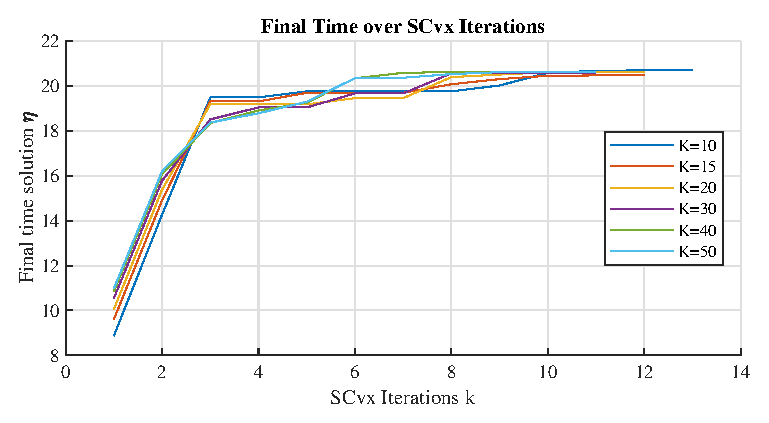
\includegraphics[width=\textwidth]{figs/iteratetiming.eps}
  \caption{Non-Planar Guidance Problem: Vehicle Approaches Offset from Target}
  \label{fig:nplanarcontrols}
\end{figure}
\begin{figure}[!htbp] 
\label{}
  \centering
  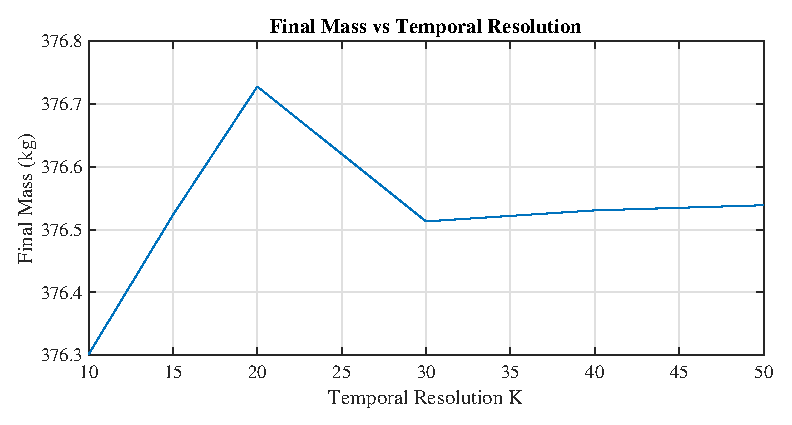
\includegraphics[width=\textwidth]{figs/massvsK.eps}
  \caption{Non-Planar Guidance Problem: Vehicle Approaches Offset from Target}
  \label{fig:nplanarcontrols}
\end{figure}
\begin{figure}[!htbp] 
\label{}
  \centering
  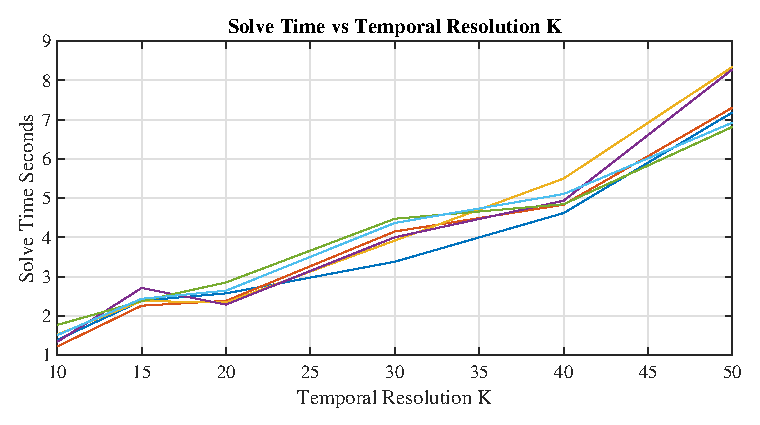
\includegraphics[width=\textwidth]{figs/solvetimevsK.eps}
  \caption{Non-Planar Guidance Problem: Vehicle Approaches Offset from Target}
  \label{fig:nplanarcontrols}
\end{figure}



\section{A Parameter Variation Study}
vary the initial conditions and plot all of these on a single plot or whatever.
do lil monte carlo
then look at runtime for different parameters etc....


\section{MRPs vs Quaternions}

\section{Corner Conditions}

\section{Glideslope and Subterminal Constraints}
